\chapter{Scoring and Ranking}
\section{Scoring Classifier}
Cambiamo ora tipo di classificatore: prima ne usavamo uno binario a cui davamo un esempio e restituiva 0 o 1, ora invece prendiamo un classificatore che prende un esempio X restituisce un vettore:
\begin{equation}
    \hat{s}: X \rightarrow \mathbb{R}^k
\end{equation}
con il vettore fatto così:
\begin{equation}
    \hat{s}=(\hat{s_1}(x),\dots,\hat{s_k}(x)).
\end{equation}
Più uno score è alto, più la classe associata a quello score, è considerata affidabile.
Se ci sono solo 2 classi, gli score negativi saranno dedicati alla classe $c_1$ e quelli positivi alla classe $c_2$.

Il training set continua ad essere un esempio con una classe associata, l'output è cambiato poichè restituisce, appunto, uno score.

\paragraph{Scoring Tree}
In questi alberi, alle foglie è associato uno score invece di una classe. Per calcolare gli score si fa il logaritmo del rapporto tra, in questo caso, spam e ham.
\begin{figure}[!h]
    \centering
    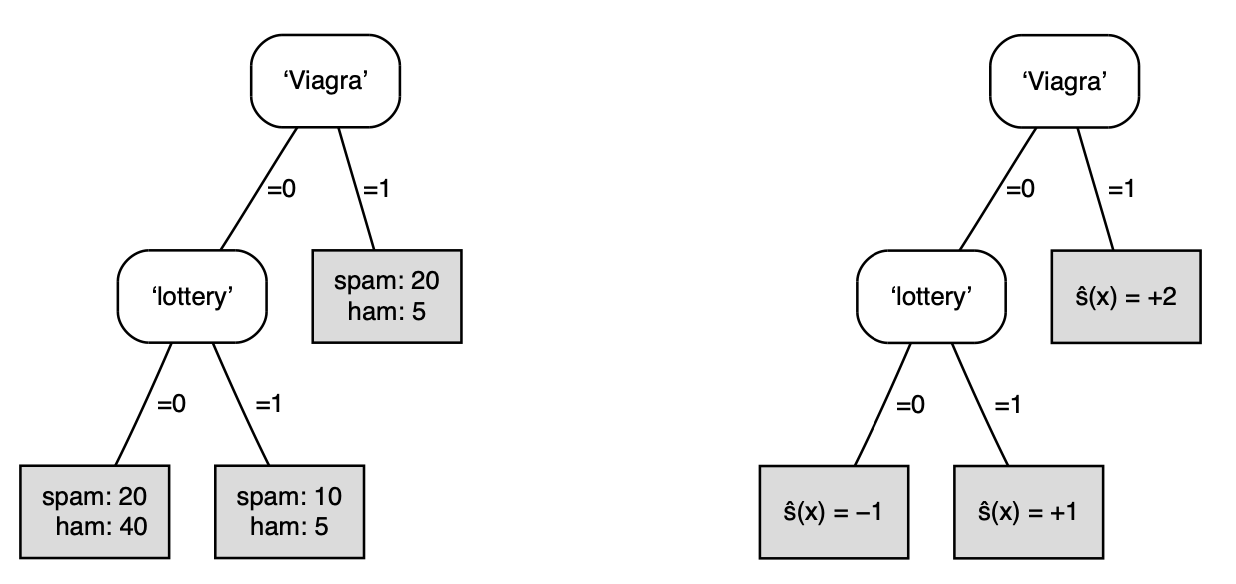
\includegraphics[scale=0.7]{images/scoringTree.png}
    \label{fig:enter-label}
\end{figure}

\paragraph{Margini.} Un \textbf{margine} è la combinazione degli score con la vera etichetta associata al modello.
\begin{equation}
    z(x)=c(x)\hat{s}(x)=\begin{cases}
        +\left|\hat{s}(x) \right| \; \text{se }\hat{s}\text{ è corretto} \\ 
        -\left|\hat{s}(x) \right| \; \text{altrimenti}
\end{cases}
\end{equation}
$c(x)$ è la classe vera che c'è nel dataset, $\hat{s}(x)$ è lo score assegnato. Per semplicità consideriamo comunque la classificazione binaria; l'idea è che il margine sia positivo quando la classificazione è corretta e negativo quando non lo è.

\paragraph{Loss function.} Una \textbf{loss function} è una funzione che misura quanto male sta facendo il modello. Spesso i problemi di apprendimento si definiscono in funzione delle loss function, come \textbf{problemi di minimizzazione della funzione}.

La funzione è definita come $L: \mathbb{R} \rightarrow [0,\infty)$ che mappa il margine $z(x)$ di un esempio ad un certo valore di loss $L(z(x))$.

Assumiamo che nel caso in cui il margine sia zero assumeremo che la loss sia $L(0)=1$. Quindi la loss sarà $L(z) \ge 1$ se $z<0$ e $0\le L(z)<1$ se $z>0$.

\begin{figure}[!h]
    \centering
    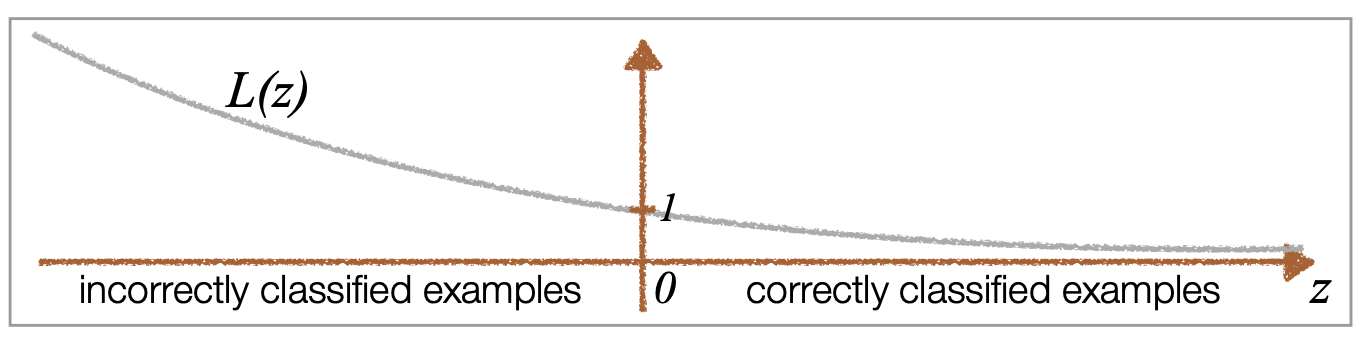
\includegraphics[scale=0.7]{images/lossFun.png}
    \label{fig:enter-label}
\end{figure}

Ci sono diversi tipi di loss function:
\begin{itemize}
    \item \textbf{0-1 loss}, la più semplice, indica che la loss è 1 se stiamo sbagliando a classificare l'esempio, 0 altrimenti
        \begin{equation}
        \begin{split}
            L_{01}(z)=1 \; \text{if} \; z\le 0 \\
            L_{01}(z)=0 \; \text{if} \; z> 0 
        \end{split}
        \end{equation}
        sommando la loss di tutti gli esempi, vediamo gli esempi che stiamo classificando male. 

        Notiamo che la funzione è discontinua
        \begin{figure}[!h]
            \centering
            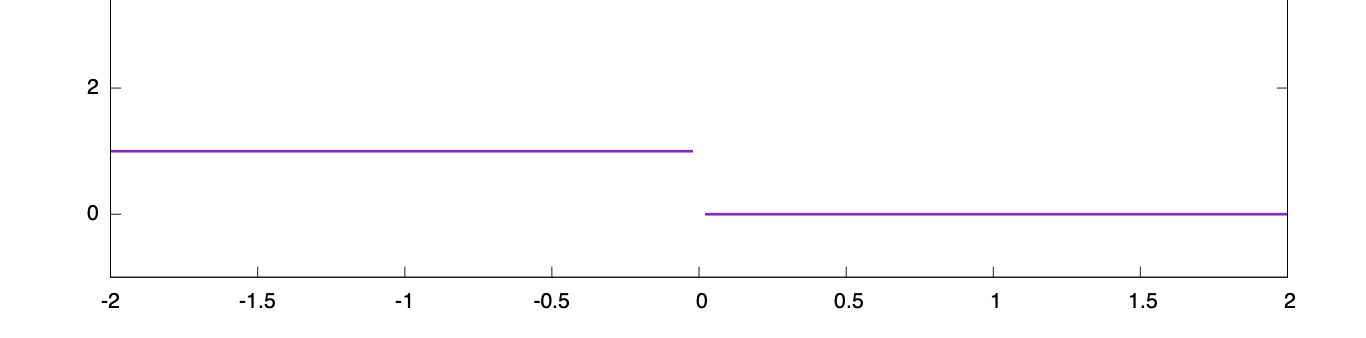
\includegraphics[scale=0.5]{images/01loss.png}
            \label{fig:enter-label}
        \end{figure}
        e la sua derivata è 0 sia a sinistra che a destra, il che vuol dire che se riesco a classificare correttamente gli esempi, non ho nessun altra informazione da utilizzare per migliorare ulteriormente il modello.
    \item \textbf{Hinge loss}, risolve parzialmente il problema della derivata,  
    \begin{equation}
        \begin{split}
            L_{h}(z)=(1-z) \; \text{if} \; z\le 1 \\
            L_{h}(z)=0 \; \text{if}\;  z> 1 
        \end{split}
    \end{equation}
    
    \begin{figure}[!h]
        \centering
        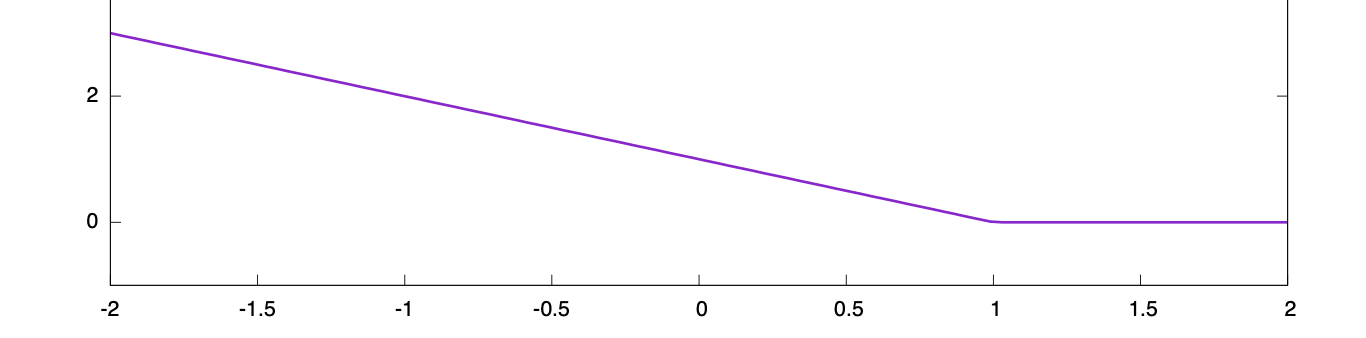
\includegraphics[scale=0.5]{images/hingeLoss.png}
        \label{fig:enter-label}
    \end{figure}
    ci permette di migliorare la classificazione anche quando siamo tra 0 e 1;
    \newpage
    \item \textbf{logistic loss}, 
    \begin{equation}
        L_{log}(z)= \log_2(1+(\exp(-z)))
    \end{equation}
    
    \begin{figure}[!h]
        \centering
        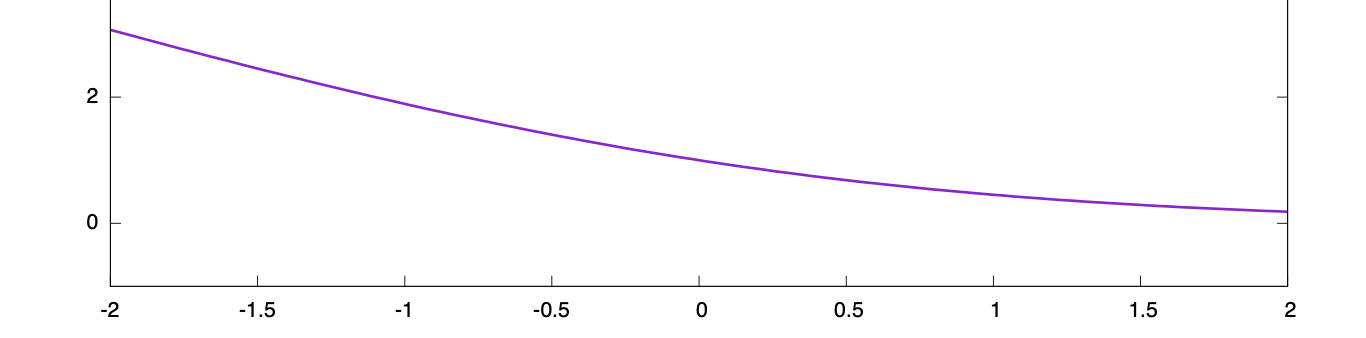
\includegraphics[scale=0.5]{images/logLoss.png}
        \label{fig:enter-label}
    \end{figure}
    è un'approssimazione della precedente, completamente continua;
    
    \item \textbf{exponential loss}, 
    \begin{equation}
        L_{exp}(z)=\exp(-z)
    \end{equation}
    
    \begin{figure}[!h]
        \centering
        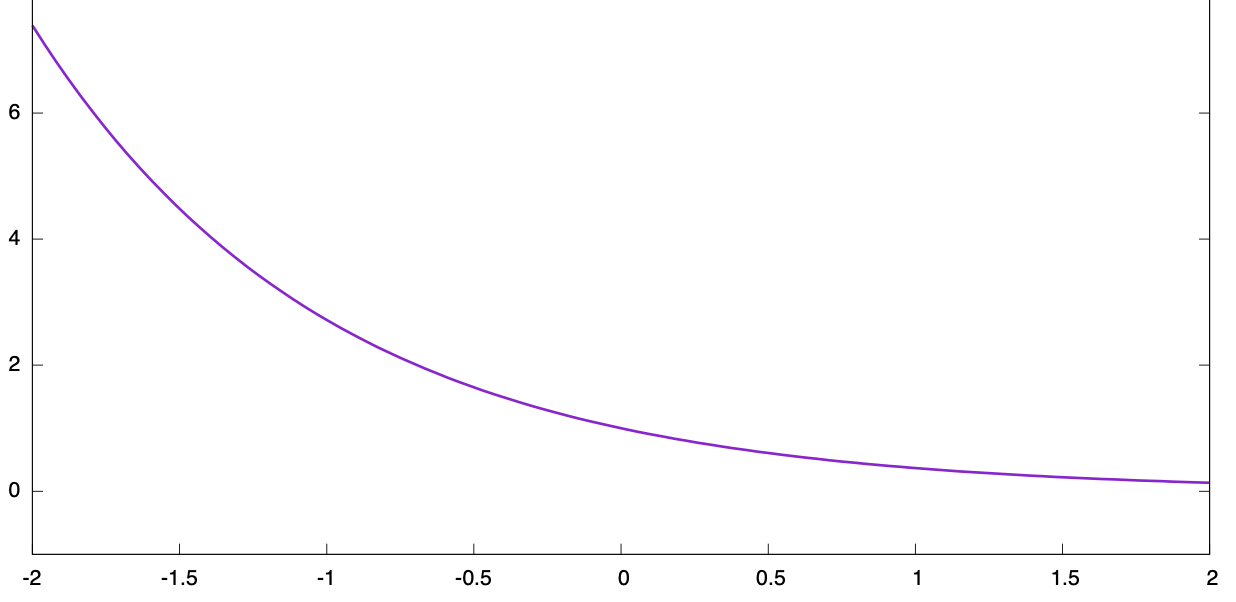
\includegraphics[scale=0.3]{images/expLoss.png}
        \label{fig:enter-label}
    \end{figure}
    \item \textbf{squared loss}, 
    \begin{equation}
        L_{sq}(z)=(1-z)^2
    \end{equation}
    
    \begin{figure}[!h]
        \centering
        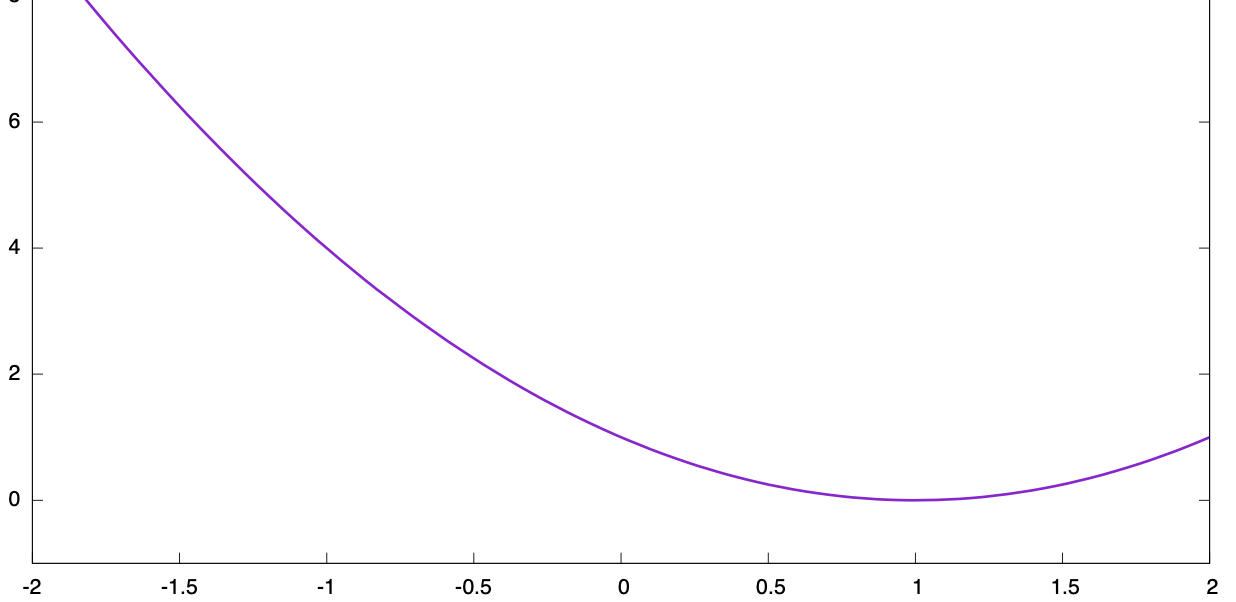
\includegraphics[scale=0.3]{images/sqLoss.png}
        \label{fig:enter-label}
    \end{figure}
\end{itemize}
Viste tutte in un unico grafico risultano l'una l'approssimazione dell'altra:
\begin{figure}[!h]
    \centering
    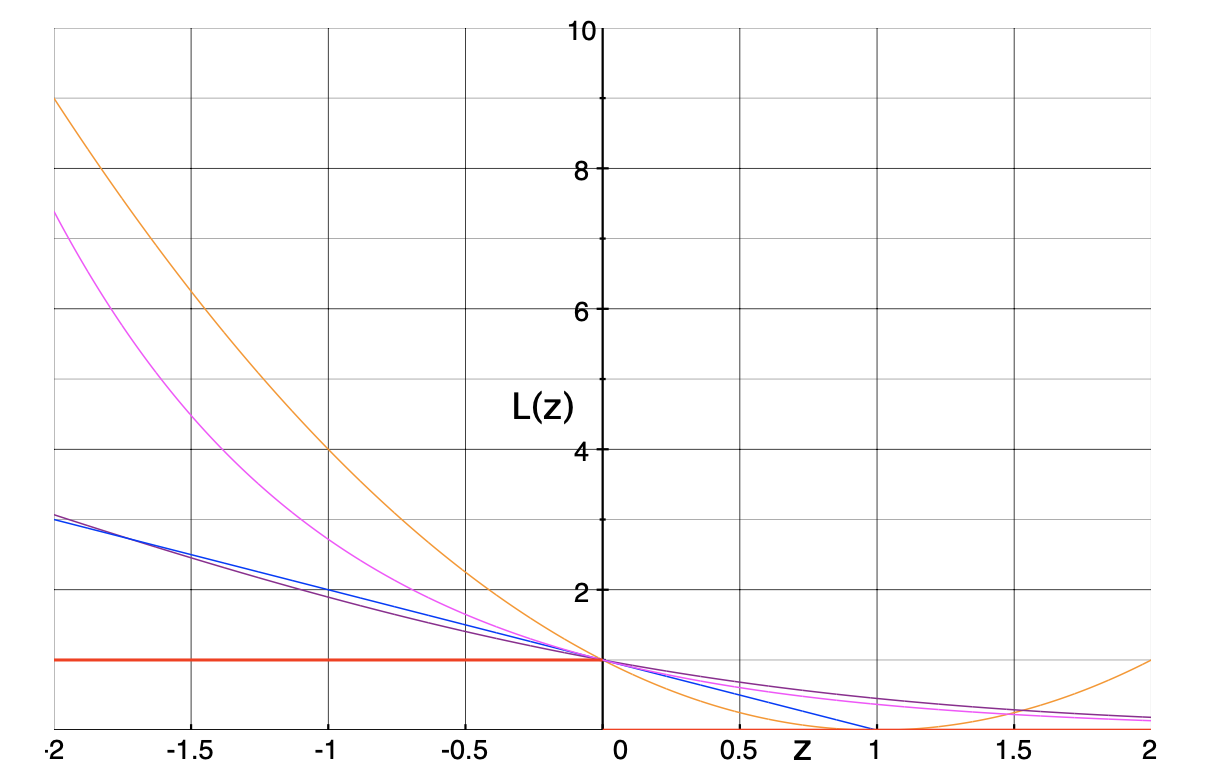
\includegraphics[scale=0.5]{images/allLoss.png}
    \label{fig:enter-label}
\end{figure}

\newpage

\section{Ranking}
Il classificatore rimane binario, ma in output v\textbf{oglio classificare le classi dalla più alla meno probabile}. Ovviamente dopo una scoring function, è facile costriure una ranking function.

Come valutiamo la bontà del ranking? Possiamo usare il \textbf{ranking error rate}, definito come:
\begin{equation}
    rank-err=\frac{\sum_{x\in Te^+,x^{'}\in Te^-}I[\hat{s}(x)<\hat{s}(x^{'})]+\frac{1}{2}I[\hat{S}(x)=\hat{s}(x^{'})]}{Pos\cdot Neg}
\end{equation}
$x$ è l'esempio positivo e $x^{'}$ è quello negativo; se lo score $x$ è più piccolo dello score di $x^{'}$ (quindi sto ordinandoli in modo sbagliato, dovrei mettere prima gli esempi positivi e poi i negativi), \textbf{aggiungo un punto d'errore} allo score che sto calcolando. \textbf{Aggiungo 0.5 punti se gli score dei due esempi sono uguali}; in questo caso non è un errore vero e proprio ma si conta come mezzo punto di errore.

Un \textbf{ranking perfetto} corrisponde ad un numeratore uguale a 0 mentre se un \textbf{ranking completamente sbagliato} è allora la parte che conta gli uguali è 0 ma l'altra è sempre vera (per ogni coppia possibile, quindi per $Pos\cdot Neg$ coppie), quindi il ranking error sarebbe uguale ad 1.

\textbf{Facciamo un esempio:}
\begin{figure}[!h]
    \centering
    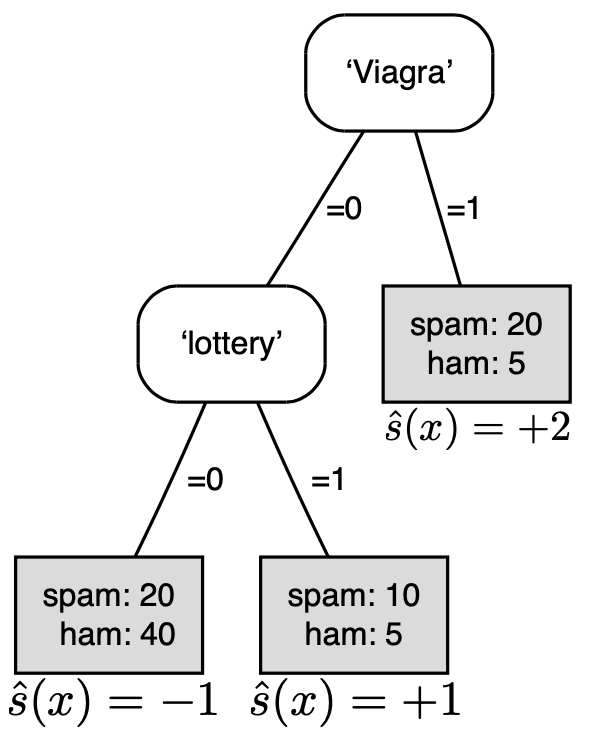
\includegraphics[scale=0.6]{images/rankError.png}
    \label{fig:enter-label}
\end{figure}


Chiameremo:
\begin{itemize}
    \item foglia 1, la foglia che ha spam:20, ham 5;
    \item foglia 2, la foglia che ha spam:20, ham 40;
    \item foglia 3, la foglia che ha spam:10, ham 5;
\end{itemize}
Cominciamo dalla foglia 1, abbiamo che quei 5 esempi negativi (ham) sono classificati in una posizione più alta rispetto ai 20 positivi (spam:20) della foglia 2 e anche rispetto ai 10 (spam:10) della 3. Lo diciamo perchè hanno uno score maggiore. Quindi $5\cdot 10 = 50$ (per la foglia 3), $5\cdot 20 = 100$ (per la foglia 2) $=150$ punti di errore.  

I 5 positivi della foglia 3 sono messi più in alto dei 20 positivi della foglia 2, quindi 100 punti di errore.

Infine calcoliamo i mezzi punti; sono 475 divisi in $20\cdot 5=\frac{100}{2}$ per la foglia 1, $20\cdot 40=\frac{800}{2}$ per la foglia 2 e $10\cdot 5=\frac{50}{2}$ per la foglia 3.

Abbiamo un totale di $475+100+150=725$ errori su 2500 esempi.

\newpage

\section{Stima delle probabilità}
Questo è un caso simile a quello dello scoring ma qui mettiamo un vincolo ulteriore agli score, imponendo che siano tutti posiviti e la loro somma sia 1. In simboli
\begin{equation}
    \hat{p}:X\rightarrow [0,1]^k
\end{equation}
con
\begin{equation}
    \hat{p}(x)(\hat{p_1}(x),\dots,\hat{p_k}(x)).
\end{equation}
Se abbiamo solo due classi, $\hat{p}(x)$ denota la probabilità stimata per la classe positiva.

\paragraph{Probability estimation tree.} Per assegnare le probabilità alle foglie, prendiamo gli esempi che ricadono in quella foglia e diciamo che la probabilità che un esempio capiti in quella foglia è data dal rapporto tra gli esempi cercati e la somma degli esempi ($\frac{20}{20+5}$ per la prima foglia).
\begin{figure}[!h]
    \centering
    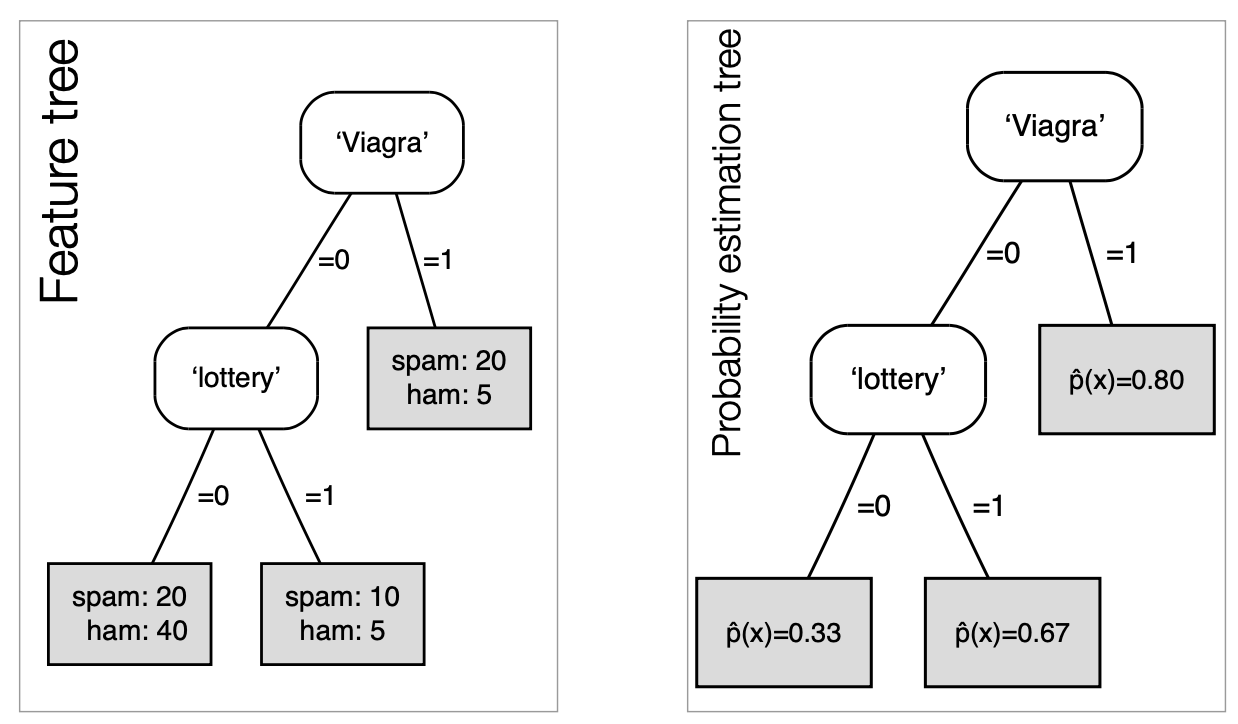
\includegraphics[scale=0.6]{images/probTree.png}
    \label{fig:enter-label}
\end{figure}

Come valuto la bontà delle probabilità emesse? Uso la \textbf{mean squared probability error}, definita così:
\begin{equation}
\begin{split}
    SE(x)=\frac{1}{2}\left|\left| \hat{p}(x)-I_c(x) \right|\right|_2^2 \\
    = \frac{1}{2} \sum_{i=1}^k(\hat{p}_i(x)-I[c(x)=C_i])^2
\end{split}
\end{equation}
dove $I_{c(x)}$ è un vettore che ha 1 nelle posizioni corrispondenti all'etichetta $c(x)$ e 0 nelle altre.

\paragraph{Esempio:}
assumiamo $\hat{p}(x)=(0.7,0.1,0.2)$ e $c(x)=C_1$ e $I_{c(x)}(1,0,0)$.
$SE(x)$ sarebbe valutata come:
\begin{equation}
    \begin{split}
        SE(x)=\frac{\left| \left| (0.7,0.1,0.2)-(1,0,0) \right| \right|_{2}^{2}}{2} \\
        =\frac{\left| \left| (-0.3,0.1,0.2) \right| \right|_{2}^{2}}{2} \\
        =\frac{0.09+0.01+0.04}{2} \\
        =\frac{0.14}{2}=0.07
    \end{split}
\end{equation}

\paragraph{}Quando lavoriamo su un intero dataset facciamo semplicemente la media degli squared error per ogni istanza
\begin{equation}
     MSE(Te)=\frac{1}{\left|Te \right|}\sum_{x\in Te}SE(x)
\end{equation}

\paragraph{Stima delle probabilità empiriche.} Dato un insieme s di esempi etichettati, possiamo stimare la probabilià delle varie classi creando il vettore $\frac{n_i}{S}$ che è il numero degli esempi etichettati con l'etichetta $n_i$ diviso la cardinalità dell'insieme:
\begin{equation}
    \dot{p}(S)=\left(\frac{n_1}{|S|},\dots,\frac{n_k}{|S|}\right)
\end{equation}

\paragraph{Correzione di Laplace.} Se alcune classi sono poco frequenti e abbiamo pochi esempi di esse, è probabile che la stima calcolata poco fa venga 0. Questo è spesso un problema perchè spesso si moltiplicano tutte le probabilità e avere uno 0 rovina tutto. Quindi cerchiamo di fare "smoothing" di queste probabilità, attraverso la correzione di Laplace. L'idea è che assumiamo di aver pescato un esempio in più per ogni classe:
\begin{equation}
    \dot{p}_i(S)=\frac{n_i+1}{|S|+k}
    \label{m-estimate}
\end{equation}

Possiamo anche non applicare uno smoothing uniforme, se in partenza sappiamo che non tutte le classi sono equiprobabili:
\begin{equation}
    \dot{p}_i(S)=\frac{n_i+m\cdot \pi_i}{|S|+m}
\end{equation}
peschiamo $m$ esempi, con $m>k$ e $\pi_i$ probabilità della classe i-esima.

La correzione di Laplace è un caso speciale della (\ref{m-estimate}) con $m=k$ e $\pi_i=\frac{1}{k}$.

